\section{Representative numerical simulations}
\label{numerical-simulations}

\subsection{General algorithm}
\label{general-algorithm}

The total Second Piola Kirchhoff stress is updated as follows
(\cite{Holzapfel:1996}, p. 3913.):

\begin{itemize}
\item Set the initial value for the stresses:
  \begin{displaymath}
    \bS_{\mathrm{vol}}^{\infty}|_{t = 0} = \bzero, \quad
    \bS_{\mathrm{iso}}^{\infty}|_{t = 0} = \bzero, \quad
    \bQ_{\alpha}|_{t = 0} = \bzero
  \end{displaymath}
\item For $t = {0, T}$:
\end{itemize}

\subsection{Modelling the experimental results of Dokos et al.}
\label{simulating-experiment}

We want to fit/compare our results with \cite{Dokos:2002}. For this,
we start with parameters from \cite{Holzapfel:2009bb}, Table 1 and
introduce additional parameters for the volumetric and viscoelastic
response.

\begin{tabular}{| c | c | r | }
  \hline
  Parameter & Unit & Value\\
  \hline
  $a$         & kPa  & 0.059\\
  $b$         &      & 8.023\\
  $a_{f}$     & kPa  & 18.472\\
  $b_{f}$     &      & 16.026\\
  $a_{s}$     & kPa  & 2.481\\
  $b_{s}$     &      & 11.120\\
  $a_{fs}$    & kPa  & 0.216\\
  $b_{fs}$    &      & 11.436\\
  $\beta$     & kPa  & 2.0e6 \\
  $\kappa$    &      & 9.000\\
  $\beta_{1}$ &      & 0.250\\
  $\tau_{1}$  & s    & 1.000\\
  \hline
\end{tabular}

\begin{figure}
  \centering
  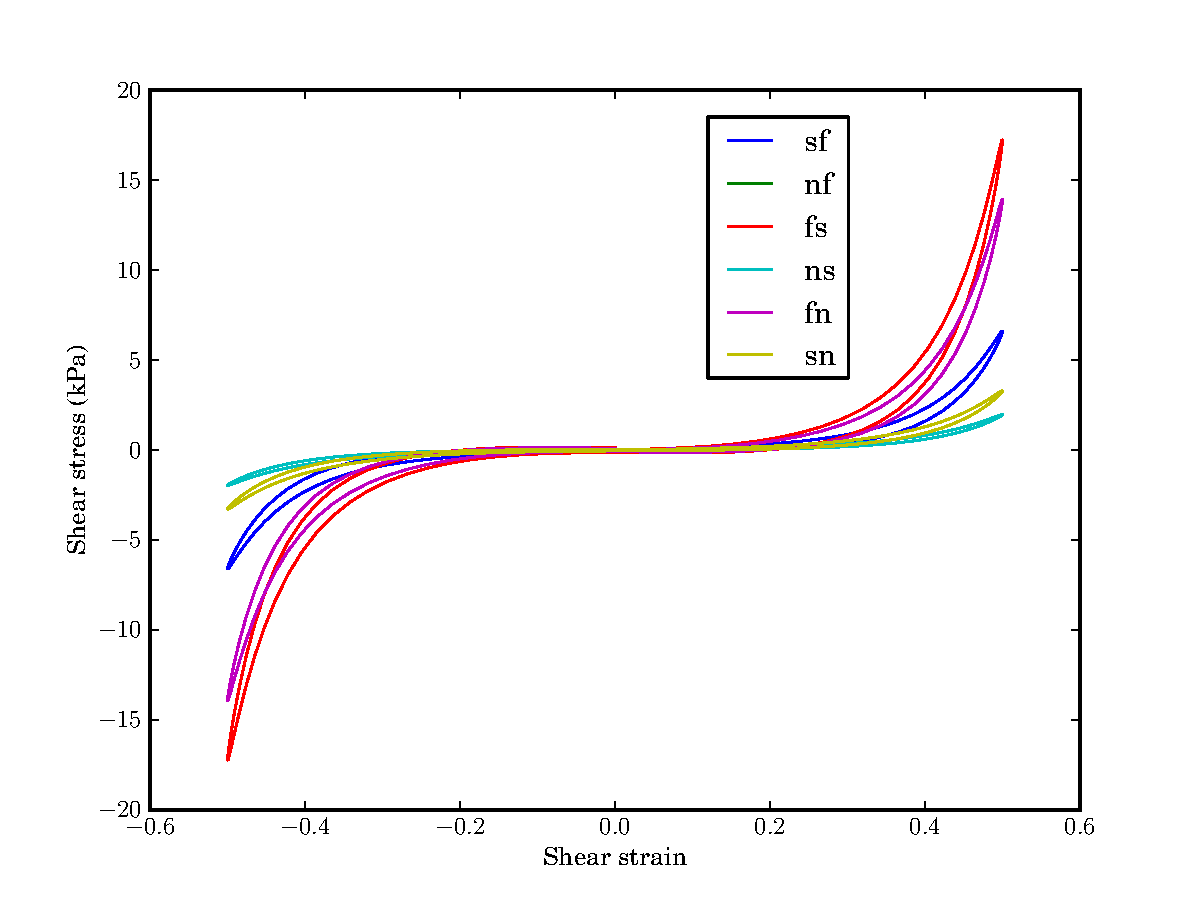
\includegraphics[width=\textwidth]
                  {images/pdf/orthotropic-viscoelasticity}
  \caption{Orthotropic viscoelastic response (analytical)}
  \label{analytica-orthotropic-viscoelasticity}
\end{figure}

%

% Local Variables:
% TeX-master: "visco"
% mode: latex
% mode: flyspell
% End:
